
\hypertarget{menu_options}{}
\section{Options}
\index{options menu}

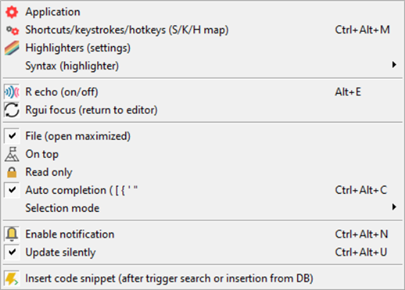
\includegraphics[scale=0.8]{./res/menu_options.png}\\

\begin{scriptsize}
  \begin{tabularx}{\textwidth}{>{\hsize=0.3\hsize}X>{\hsize=0.7\hsize}X}\\
    \hline
    \textbf{Option} & \textbf{Description} \\
    \hline
    Application & Opens the \href{\#working\_app\_main}{Application options} dialog \\
    Shortcuts/keystrokes/hotkeys (SKH map)& Opens the \href{\#working\_shortcuts}{Shortcuts customization} dialog \\
    Highlighters (settings) & Opens the \href{\#working\_highlighters}{Highlighters (settings)} dialog \\
    Syntax (highlighters) & \textit{\href{\#menu\_options\_syntax}{See options ...}} \\
    \hdashline[1pt/1pt]
    R echo (on/off) & Toggles R echo option (file, selection, clipboard, block, contiguous and lines to end page) \\
    Rgui focus (return to editor) & When this option is set the focus will go back to the active
     editor after any Send or Control action \\
    \hdashline[1pt/1pt]
    File (open maximized) & When this option is set all files will be opened maximized \\
    On top & Toggles Tinn-R's ability to be the topmost window on the desktop \\
    Read only & Toggles file read-only status. When set as read-only the file name on the file
     tab is among \texttt{$<$}...\texttt{$>$} \\
  		Auto completion & Toggles auto completion resource \\
    Selection mode & \textit{\href{\#menu\_options\_selectionmode}{See options ...}} \\
    \hdashline[1pt/1pt]
    Enable notification & Toggles file notification resource \\
  		Update silenty & Toggles update silenty resource \\
    \hdashline[1pt/1pt]
    Insert code snippet (after trigger search or insertion from DB) & If this option is not checked, after a search
     via Search trigger or insertion via tools/database/snippets, only the trigger is inserted. Otherwise the trigger
     is inserted and immediately replaced with the corresponding block of text \\
    \hline
  \end{tabularx}
\end{scriptsize}


\hypertarget{menu_options_syntax}{}
\subsection{Syntax (highlighter)}
\index{options menu!syntax}

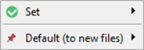
\includegraphics[scale=0.8]{./res/menu_options_syntax.png}\\

\begin{scriptsize}
  \begin{tabularx}{\textwidth}{>{\hsize=0.3\hsize}X>{\hsize=0.7\hsize}X}\\
    \hline
    \textbf{Option} & \textbf{Description} \\
    \hline
    Set & \textit{\href{\#menu\_options\_syntax\_set}{See options ...}} \\
    \hdashline[1pt/1pt]
    Default (to new files) & \textit{\href{\#menu\_options\_syntax\_default}{See options ...}} \\
    \hline
  \end{tabularx}
\end{scriptsize}


\newpage
\hypertarget{menu_options_syntax_set}{}
\subsubsection{Set:}\\
\index{options menu!syntax set}

\includegraphics[scale=0.8]{./res/menu_options_syntax_set.png}\\

\begin{scriptsize}
  \begin{tabularx}{\textwidth}{>{\hsize=0.2\hsize}X>{\hsize=0.8\hsize}X}\\
    \hline
    \textbf{Option} & \textbf{Description} \\
    \hline
    All & File without extension or not recognized extension \\
    Assembly x86 & x86 Assembly files \\
    Bath MS\_DOS & MS\_DOS Bath files \\
    C\# & C\# files \\
    C/C++ & C/C++ files \\
    CSS & Cascading SS files \\
    Fortran & Fortran files \\
    Haskell & Haskell files \\
    HTML & Hypertext Markup Language (HTML) files \\
    HTML complex & Hypertext Markup Language (HTML) complex (HTML \& JavaScript) files \\
    INI & INI files \\
    Java & Java files \\
    JavaScript & JavaScript files \\
    Object Pascal & Pascal files \\
    Perl & Perl files \\
    PHP & PHP files \\
    PHP complex & PHP (HTML \& JavaScript \& PHP) complex files \\
    Python & Python files \\
    R & R files \\
    R complex & R complex (R \& URI) files \\
    R doc & Rd files \\
    R html & Rhtml files \\
    R markdown & Rmd files \\
    R noweb & R noweb (TeX \& R) files \\
    Ruby & Ruby files \\
    SQL & SQL files \\
    Structured Text & Structured Text files \\
    TclTk & TclTk files \\
    TeX & TeX files \\
    Text & Text files \\
    URI & Uniform Resource Identifiers (URI) files \\
    MS VBScript & MS VBScript files \\
    Visual Basic & Visual Basic files \\
    XML & XML files \\
    \hline
  \end{tabularx}
\end{scriptsize}

If necessary select manually one of the list. Tinn-R recognizes
automatically the syntax based on the file extensions.


\hypertarget{menu_options_syntax_default}{}
\subsubsection{Default (to new files):}\\
\index{options menu!default}

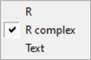
\includegraphics[scale=0.8]{./res/menu_options_syntax_default.png}\\

\begin{scriptsize}
  \begin{tabularx}{\textwidth}{>{\hsize=0.2\hsize}X>{\hsize=0.8\hsize}X}\\
    \hline
    \textbf{Option} & \textbf{Description} \\
    \hline
    R & When this option is set the highlighter of all new files will be set as \textit{R} \\
    R complex & When this option is set the highlighter of all new files will be set as \textit{R complex} \\
    Text & When this option is set the highlighter of all new files will be set as \textit{Text} \\
    \hline
  \end{tabularx}
\end{scriptsize}


\hypertarget{menu_options_selectionmode}{}
\subsection{Selection mode}
\index{selection mode menu}

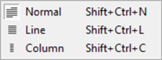
\includegraphics[scale=0.8]{./res/menu_options_selectionmode.png}\\

\begin{scriptsize}
  \begin{tabularx}{\textwidth}{>{\hsize=0.3\hsize}X>{\hsize=0.7\hsize}X}\\
    \hline
    \textbf{Option} & \textbf{Description} \\
    \hline
    Normal & \href{\#working\_selectionmode\_normal}{See selection type normal ...} \\
    Line & \href{\#working\_selectionmode\_line}{See selection type line ...} \\
    Column & \href{\#working\_selectionmode\_column}{See selection type column ...} \\
    \hline
  \end{tabularx}
\end{scriptsize}
